\chapter{Metoder}
Dette kapitel indeholder beskrivelser af hvordan projektet er udført, og med hvilke metoder der er brugt. Yderligere indeholder kapitlet projektstyring, samt hvilke modeller der er fulgt igennem projektforløbet. 

\section{Samarbejdsaftale}
For at gruppens medlemmer var enige fra starten af projektet, om blandt andet arbejdsindsats, samt timer der skulle bruges på projektet blev der lavet en samarbejdsaftale. Se samarbejdsaftalen i bilag XX

\section{Samarbejdspartnere}
Gruppens kunde er Søren Gregersen, overlæge på Medicinsk Endokrinologisk Afdeling, Aarhus Universitetshospital. Det er i samarbejde med Søren at projektet er blevet specificeret, samt hvilke krav der er til den endelige prototype.
Samuel Alberg Thrysøe er gruppens projektvejleder. Der er afholdt ugentlige vejledermøder, hvor gruppen har givet status på projektet og hvor der er diskuteret forskellige problemstillinger. 
Simon Vammen Grønbæk og Karl-Johan Schmidt har fungeret som projektets review gruppe. Der er holdt møde hver tredje uge omhandlende aftalt dagsorden. Formålet med review gruppen er at få konstruktiv feedback på evt. rettelser, opbygning af rapport og generel forståelse. Review gruppen har været gode til at sparre med omkring diskussioner, samt andre tvivl spørgsmål i gruppen. Derudover har det også gjort at deadlines har været mere faste, da review gruppen også har været afhængige af datoen.
Til hvert vejledermøde har der været dagsorden med punkter, som formål og begrundelse for punktet på dagsorden. Dagsorden er sendt til vejleder senest en dag før vejledermødet, dette er gjort for at give vejleder en chance for at forberede sig på den givne dagsorden. Til hver vejledermøde er der udført et referat som kan ses i bilag XX. 

Reviewsmøderne har foregået på en lignede måde med vejledermøderne. Der er lagt en dagsorden for hver gruppe hvad der skulle reviews, hvor efter dokumenterne er udvekslet mellem de to grupper. Grupperne har skrevet kommentar til dokumentet, hvorefter kommentarene og rettelserne er diskuteret på møderne. 

\newpage
\section{Udviklingsværktøjer}
Dette afsnit består af en kort beskrivelse omkring udviklingsværktøjerne brugt i projektet.

\textbf{MATLAB:} Softwaren til systemet er udviklet i MATLAB. Versionen der er anvendt er R2015b. Tilføjelsespakker brugt i projektet er følgende:
\begin{itemize}
\item Arduino Support Package (14.2.2)
\item Webcam Support Package (15.2)
\end{itemize}
Disse pakker anvendes til, at interagere med Arduinoen og USB mikroskopet. 

\textbf{Fritzing:} Fritzing er brugt til at illustrere kredsløbsdiagrammer(schematics), samt enhedstest af hardwaren ved illustrationer af \textit{fumlebræt}. Hvilket har været en stor hjælp til dokumentationen af netop til enhedstestene. Derudover har det også været med til at huske tidligere opstillinger der er brugt på \textit{fumlebræt}, for at de nemt kan genskabes.

\textbf{Eagle:} Eagle et program til at lave print layouts med. Det er brugt til at lave et samlet PCB layout for hardware elementerne. I \textit{Eagle} er der generet gerber filer, som er sendt til PCB fabrikanten.

\textbf{SolidWorks:} Er et program til, som kan illustrer mekaniske 3D modeller. Er brugt til at lave kamerahuset med, for senere at  få det 3D printet.

\textbf{Arduino IDE:} Er programmet som er udbudt af Arduino til at programmere arduino udviklingskortet. \textit{Arduino IDE} er i projektet brugt til enhedstest til at teste hardware opstillingerne med. 

\textbf{Microsoft Visio:} Microsoft Visio er et tegne program, som kan bruges til at illustrere forskellige modeller. Gruppen har brugt det til at lave udviklingsdiagrammer, samt illustrationer med. 

\textbf{Latex/texmaker:} Er brugt til at skrive alt dokumentationen i projektet. \textit{Textmaker} gør det muligt at arbejde på samme dokument samtidigt, hvilket har været en stor hjælp.

\textbf{Pivotaltracker:} Er et SCRUM baseret projektstyrings program, der hjælper med at styre arbejdsressourcerne til projektet. Der er i afsnittet \ref{subsec:agil} uddybet hvordan \textit{Pivotaltracker} er brugt i projektet.

\textbf{Github:} Er et versionsstyrings program, i projektet er det brugt til versionsstyring af dokumenter og koden til projektet. Se afsnit \ref{subsec:github} for uddybende dokumentation omkring \textit{Github} er brugt.

\textbf{Dropbox:} Er et delings program der ligger i "skyen". I projektet er dropbox brug til gemte artikler, diagrammer, billeder og generelle noter.

\textbf{Microsoft Onenote:} Er et program til at lave noter i. I projektet er programmet brugt til at have fælles noter og huskelister.

\fxnote{flere?}
\newpage
\section{Versionsstyring}
I projektet er der gjort brug af versionsstyrings softwaren \textit{GitHub}. Til store ændringer har dokumenterne fået et nyt versions nummer og versionshistoriks tabellen er opdateret i hvert dokument, se tabellen nedenfor. 

\begin{center}
		\begin{longtable}{ | m{1.5cm} | m{2cm}| m{7cm}| m{2cm}| } 
			\hline
			\textbf{Version}  & \textbf{Dato} & \textbf{Beskrivelse} & \textbf{Initialer}  \\ 
			\hline
			0.1  &  19/09 2015  & Dokument sendt til review & AE og AT \\
			\hline
		1.0  &  19/09 2015  & Rettelser fra reviewmøde og Latex layout & AE og AT \\
		\hline
		1.1  &  20/10 2015  & Kamera krav tilføjet & AE og AT \\
		\hline
		2.0  &  6/11 2015  & Definitioner og layout ændringer & AE og AT \\
			\hline
		\end{longtable}
		
	\end{center}


\subsection{Github}
\label{subsec:github}
Til versionsstyring af projektdokumentationen og source kode anvendes GitHub, som bygger på open source versions styrings systemet Git. Her opdateres der løbende ændringer, så det nyeste dokumentation og source kode altid er tilgængeligt. 
Som user interface til GitHub anvendes GitHub Desktop (figur: \ref{fig:git}). I GitHub Desktop vises en tidslinje, for hvornår der er lavet ændringer. Under de enkelte filer kan man se hvad der er ændret i for den gældende version. Programmet giver yderligere indblik i hvilke filer der lokalt er lavet ændringer i, som ikke er tilføjet repositoriet endnu.
\begin{figure}[H]
	\centering
	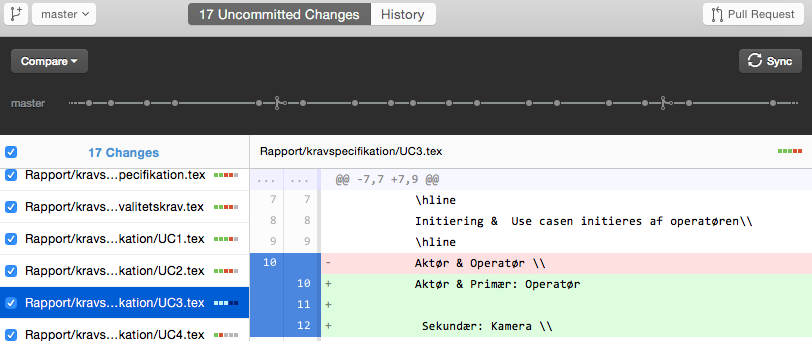
\includegraphics[width=1\textwidth]{billeder/github.png}
	\caption{GitHub Desktop}
	\label{fig:git}
\end{figure}
\newpage

\section{Projektstyring/planlægning} 
Til projektstyring af dette projekt er der brugt en stage gate model. En stage gage model(figur \ref{fig:stage-gate}) er bestående af nogle udviklingsfaser(stages), hvor ved der er en deadline for de konkrete faser. For at komme til næste fase/stage, skal der være opfyldt nogle kriterier. Kriterierne sættes op i en tjekliste(se figur \ref{fig:stage-gate-tjekliste}), hvor de kan krydses af. Alle punkter skal være opfyldt for at komme i gennem gaten. En stage gate model er god til at få et produkt på markedet, men det har sine svagheder ved en agil udviklingsprocess. Derfor er der i projektet arbejdet med åbne gates, det vil sige at der har været mulighed for at gå tilbage for at justerer på dokumenter.

%\begin{landscape}
\begin{figure}[H]
	\centering
	\includegraphics[width=0.66\textwidth]{billeder/Hovedrapport/Stage-gatel.PDF}
	\caption{Stage gate model}
	\label{fig:stage-gate}
\end{figure}
%\end{landscape}
\fxnote{stage gate modellayout}

\begin{figure}[H]
	\centering
	\includegraphics[width=0.7\textwidth]{billeder/Hovedrapport/Stagegatetjekliste.PDF}
	\caption{Stage gate tjekliste}
	\label{fig:stage-gate-tjekliste}
\end{figure}

%\begin{sidewaysfigure}
%\begin{figure}[H]
%	\centering
%	\includegraphics[width=0.6\textwidth]{billeder/Hovedrapport/Stage-gateP.PDF}
%	\caption{Stage gate model}
%	\label{fig:moscow}
%\end{figure}
%\end{sidewaysfigure}



%\begin{figure}
%  \begin{sideways}
%    \begin{minipage}{27.5cm}
%      \includegraphics[width=0.6\textwidth]{billeder/Hovedrapport/Stage-gateP.PDF}
%    \end{minipage}
%  \end{sideways}
%  \centering
%  \caption[Caption]{Caption.}
%  \label{pic:picture}
%\end{figure}

\subsection{Agil udviklingsprocess}
\label{subsec:agil}
I projektet er der brugt en agil arbejdsprocess hvor der konstant er fokus på at målrette og prioritere arbejdet mod det, der har givet mest værdi for projektet og kunden. Det vil sige at der løbende er prioriteret mellem opgaverne, hvorefter delopgaver er blevet revurderet og planlagt. Dette gør at produktet og resultater evalueres og testes løbende, hvilket har dannet grundlag for prioriteringen af opgaverne til næste periode(sprint). Til at sikre arbejdsressourcerne, der har været tilrådighed, er blevet brugt på den mest effektive måde i projektet, er der brugt elementer fra SCRUM. SCRUM er en iterativ arbejdsmetode, hvor  der er iterationer(sprints), som i dette projekt har haft en periode på en uge. SCRUM er implementeret i projektet vha. \textit{Pivotaltracker}. 

I Pivotaltracker defineres projektets arbejdsopgaver, hvorefter de tildeles point alt efter hvor stor arbejdsbyrden er. De enkelte opgaver prioriteres herefter i projektets backlog, hvor Pivotaltracker automatisk tilføjer opgaver til den igangværende sprint udfra den nuværende “velocity”. Et nyt sprint påbegyndes automatisk når en ny uge starter.

Det betyder, at der er fuldstændig styr på om projektet går for langsomt, eller om udviklingen af projektet er godt med. Dette kan holdes op i mod den tidligere nævnte stage gate model.

Herudover giver Pivotaltracker mulighed for en komplet log over projektets udførte opgaver og afsluttede sprints. Her kan man se hvilke opgaver der er udført i hvilken uge. I projektet anvendes dette som logbog over udførte arbejdsopgaver.

En opgave kan have forskellige states, som definerer dens status. Når en opgave er afsluttet kan den afleveres til review, hvor den herefter enten kan godkendes eller afvises. Dette er særligt anvendeligt i projektets udviklingsfase, hvor en feature kan testes og godkendes af et andet projektmedlem. Figur \ref{fig:pt_sprints}  viser et overblik over tidligere sprints, hvor figur \ref{fig:pt_currentsprint} viser en igangværende sprint med opgaver der er godkendt, afsluttet og ikke færdiggjorte endnu.

\begin{figure}[htbp] \centering
\begin{minipage}[b]{0.48\textwidth} \centering
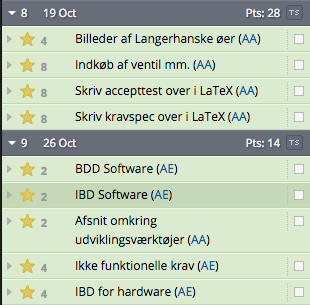
\includegraphics[width=1.00\textwidth]{billeder/pt_previous_sprints} % Left picture
\end{minipage} \hfill
\begin{minipage}[b]{0.48\textwidth} \centering
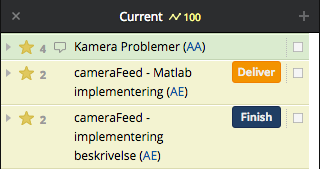
\includegraphics[width=1.00\textwidth]{billeder/pt_current_sprint} % Right picture
\end{minipage} \\ % Captions og labels
\begin{minipage}[t]{0.48\textwidth}
\caption{To færdiggjorte sprints} % Left caption and label
\label{fig:pt_sprints}
\end{minipage} \hfill
\begin{minipage}[t]{0.48\textwidth}
\caption{Igangværende sprint} % Right caption and label
\label{fig:pt_currentsprint}
\end{minipage}
\end{figure}
\fxnote{overvej om vi skal have andre billeder med en højere vilocity}

\section{Udviklingsfaserne}
Under udviklingen af projektet, er der gennem gået fire faser. Den første fase i projektet har været koncept analyse. Koncept analysen bestod af litteratursøgning omkring langerhanske øer, dette blev gjort for at opnå tilstrækkelig viden omkring størrelserne, deres egenskaber mm. Der blev også søgt allerede eksisterende sorteringsmetoder, som blev anvendt på det daværende tidspunkt. Dette var primært for at opnå erfaring inden for området på kort tid. Efter litteratursøgningen blev et overordnet koncept etableret i samarbejde med kunden(\textit{Søren Gregersen}). Samtidigt med koncept analysen, blev der parallelt med, tænkt på produktionen af produktet. Det er gjort for at undgå løsninger, som ikke kan produceres eller er besværlige at fremstille. 

Den anden fase består af kravspecifikationen, hvilket er udarbejdet i tæt samarbejde med kunden. En kravspecifikation sikre at kunde og projekt udviklere er enige om projektets udformning. I kravspecifikationen er der brugt usecasediagram, samt fully dressed beskrivelser til hver usecase. Der laves fully dressed, for at klaregøre normal forløbet for hver usecase, samt undtagelser og udvidelser til dem. Derudover er det også i kravspecifikationen. at der er specificeret ikke funktionelle krav og kvalitetskrav. Samtidigt med kravspecifikationen er der udarbejdet en accepttest. Denne test er med til at verificere at alle krav, der er bestemt i samarbejde med kunden er opfyldte. I accepttesten er det beskrevet hvordan hver enkelt krav skal testes. Accepttesten udføres før produktet afleveres til kunden. Se afsnit \ref{subsec:krav} for eksempler.

Den tredje fase i projektet har været designfasen, hvor der udfra kravspecifikationen er lavet overordnede diagrammer. Diagrammerne er brugt til at beskrive systemet overordnet, men også i små delsystemer. Det er diagrammerne der er brugt til at videre udvikle systemet. Desuden er de enkelte komponenters specifikationer beskrevet i designdokumentet. Derfor er det i denne fase der er bestilt komponenter til projektet. Se afsnit \ref{subsec:design} for eksempler. Efter denne fase blev det klart for gruppen, at der skulle bruges mere tid for at opnå målet defineret fra starten. Derfor blev der iværksat en handlingsplan for projektet, som kan ses i BILAG XX. De primære dele af handlingsplanen består i øge arbejdsressourcerne til 50 timer i ugen. hvilket også kan ses i \textit{pivotaltracker}, hvor målet \textit{Velocity} har været 100point. 

I den fjerde fase er der blevet produceret en prototype. Derfor er der i denne fase kodet, monteret og testet. Denne fase er sket efter en iterativ proces, så der først kodes, monteres og derefter testes det. Dette er gjort ved så små delelementer som muligt, for at være sikker på at hver delelement virker inden det sættes sammen. Se afsnit \ref{subsec:Implement} for eksempler af denne fase. 

De fire udviklings faser brugt i projektet kan illustreres som på figur \ref{fig:v-model}. Modellen har sine fordele og ulemper. Fordelene er at der sikres dokumentation af projektet fra starten, samt at der hele tiden tænkes på slutresultatet og slutbrugeren. Ulemperne er at der er meget dokumentation, der bliver ændret fra hvad det var i starten af projektet. På den måde kan man godt tro at det er spild af tid, men det sikre samtidigt at projektet bliver vel dokumenteret og gennemtænkt fra starten.

\begin{figure}[H]
	\centering
	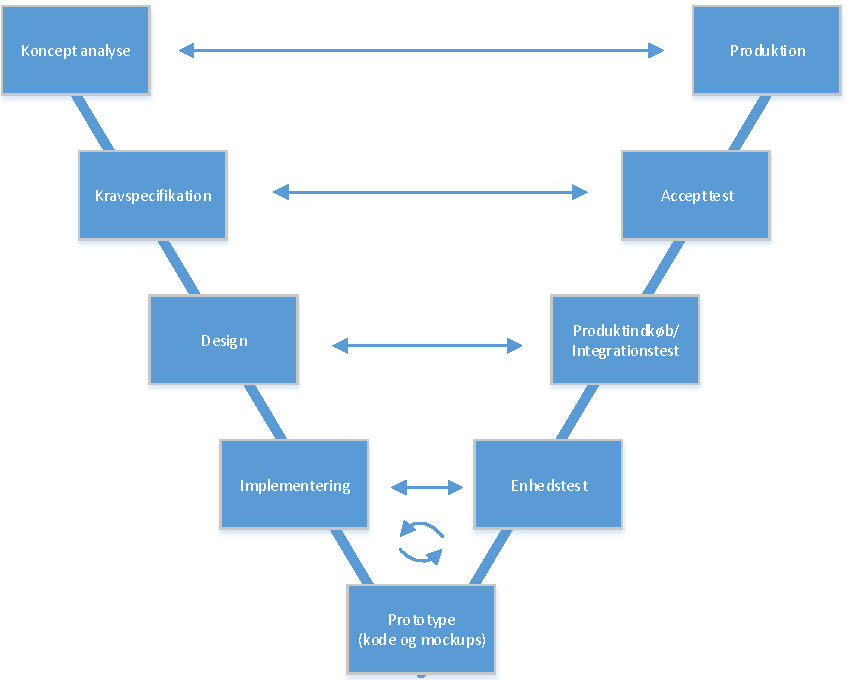
\includegraphics[width=0.7\textwidth]{billeder/Hovedrapport/V-model.PDF}
	\caption{V-model}
	\label{fig:v-model}
\end{figure}

I modsætning til v-modellen findes der også vandfaldsmodellen, hvor hver enkelt fase bliver lavet færdig før næste fase påbegyndes. Dette medfører ofte nedprioritering af test og andre sene deadlines i projektet, grundet at tidligere tidsplaner er overskredet.
\newpage

\section{Første udviklingsfase: koncept analyse}
For at eftervise at der er brugt de beskrevne metoder ovenfor, er der valgt at tage eksempler med i rapporten. I afsnittet er der eksempler fra hver udviklingsfase,  %for at eftervise de fire udviklingsfaser projektet har været i gennem.
 
\section{Anden udviklingsfase: Kravspecifikation og accepttest}
\label{subsec:krav}
For at vise et eksempel for den anden udviklingsfase i projektet, er der valgt at tage \textit{Aktør beskrivelse}, det over ordnet \textit{use case diagram}, samt et \textit{fully dressed use case} og et udpluk fra accepttesten


\subsection{Aktør beskrivelse}
Systemets primære aktør er operatøren, som står for påfyldning af celler, start og stop af sorteringsprocessen. Operatøren har mulighed for at interagere med systemet via en grafisk brugergrænseflade. Systemets sekundære aktør er kameraet og PC’ens filsystem. Kameraet er systemets interface til detektion af de Langerhanske øer. Filsystemet er hvor der løbende gemmes en log over sorteringsprocessen.

\subsection{Use Case Diagram}
I Use Case diagrammet (figur: \ref{fig:usecase}) er der vist, hvilke use cases systemet \textit{The Cell Collector} består af. Yderligere er det vist, hvilke aktører der initiere de enkelte use cases. På venstre side er systemets primære aktør \textit{operatøren} vist, mens systemets sekundære aktører \textit{kamera} og \textit{database} er placeret i højre side. 

\begin{figure}[H]
	\centering
	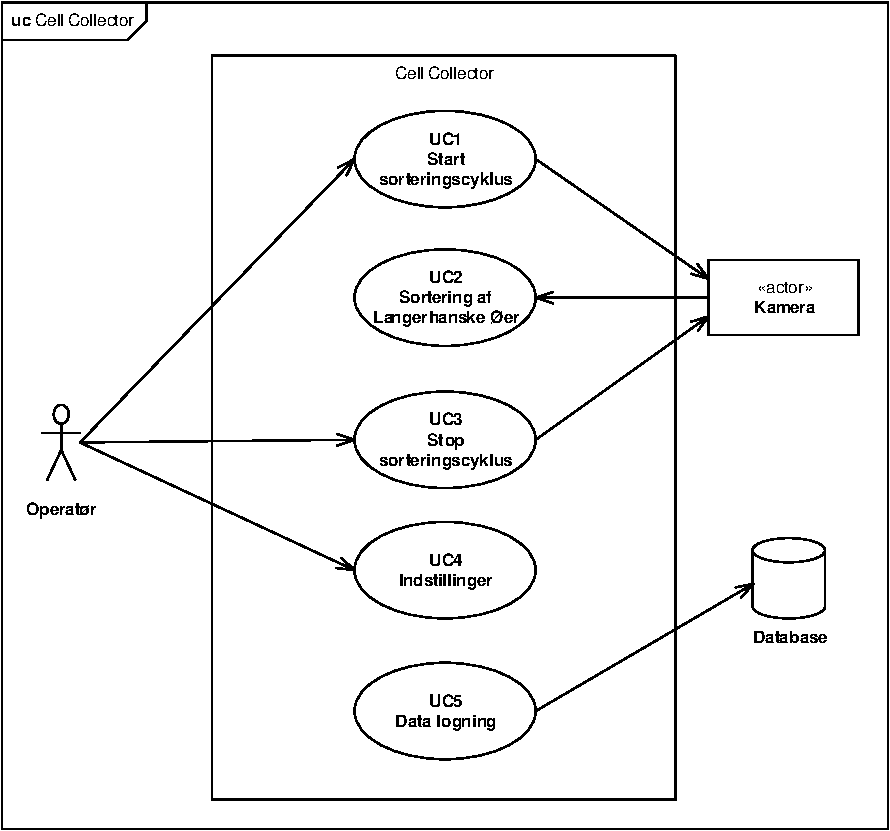
\includegraphics[width=1\textwidth]{billeder/UC_CellCollector.pdf}
	\caption{Use Case diagram for The Cell Collector}
	\label{fig:usecase}
\end{figure}

Efter use case diagrammet var færdigt, blev der udarbejdet fully dressed use cases som kan ses på nedenstående tabel. Tabellen beskriver normalforløbet og undtagelser for \textit{Sortere langerhanske øer}. 

\newpage 
\subsection{Fully dressed use case for use case1}
\begin{center}
		\begin{longtable}{ | m{4cm} | m{8cm}| } 
			\hline
			Mål & Start sorteringscyklus \\ 
			\hline
			Initiering &  Use casen initieres af operatøren\\
			\hline
			Aktør & 
			Primær: Operatør
			
			 Sekundær: Kamera			  \\ 
			\hline
			Startbetingelser & The Cell Collector programmet er startet på computeren \\ 
			\hline	
			Slutbetingelser ved succes & Systemet starter med sorteringen af Langerhanske øer \\
			\hline
			Slutbetingelser ved undtagelse & N/A \\
			\hline
			Normalforløb & \begin{enumerate}
				%\setlength\itemsep{0cm} % Decrease line distance
				\item Operatør fylder celleopløsningsbeholderen
				\item Celleopløsningsbeholderen er fyldt
				\item Operatør starter sorteringscyklus ved at klikke på [Start]
				\subitem [Undtagelse 1: Wastebeholder er fyldt] 
				\item Systemet initialiserer Arduinoen
				\subitem [Undtagelse 2: Ingen forbindelse til Arduino]
				\item Systemet kontrollerer celleopløsningsbeholderen ved at konvertere spændingen (\SI{}{\volt})  til \SI{}{\milli\litre}, og vise beholderens indhold (\SI{}{\milli\litre}) på GUI
				\item Systemet initialiserer kameraet
				\subitem [Undtagelse 3: Kameraet initialiserer ikke]
				\item Systemet tænder for kamera lyset
				\item Systemet tænder for pumpen
				
			\end{enumerate} \\ 
			\hline
			Undtagelser & [Undtagelse 1: Wastebeholder er fyldt] 
			
			\begin{enumerate}
			\item Systembesked: Tøm venligst Wastebeholder før start
			\item Operatøren trykker “OK”
			\item Systemet fortsætter opstartprocessen
			\end{enumerate} 
			
			[Undtagelse 2: Ingen forbindelse til Arduino]
			
			\begin{enumerate}
			\item 1.	Systembesked: Ingen forbindelse til Arduino, kontrollér forbindelser.
			\end{enumerate} 
	
			[Undtagelse 3: Kameraet initialiseres ikke]
			
			\begin{enumerate}
			\item System fejlmeddelse: Kameraet er ikke initialiseret:
			\item Genstart initialisering af Kameraet
			\end{enumerate} \\
			\hline
		\end{longtable}
		
	\end{center}

Efter at normalforløbet og undtagelserne er defineret, blev accepttesten lavet for den givne use case. Til hvert punkt i normalforløbet er der forberedt en test, som indeholder et krav nr, handling dvs det der skal gøres for at starte testen. Derudover er der \textit{forventet resultat}, som skal ske for at testen kan godkendes. Testmetode beskriver hvordan testen skal udføres og hvordan den godkendes. Denne test er et udsnit af accepttesten , som er udarbejdet i samarbejde kunden.

\subsection{Accepttest for krav 1.3}
	\begin{center}
		\begin{longtable}{ | m{4cm}| m{8.5cm}|} 
			\hline
			\textbf{Krav nr.} & 1.3    \\ 
			\hline
			\textbf{Handling} &  Operatør starter sorteringscyklus ved at klikke på [Start]  \\
			\hline
			\textbf{Forventet resultat} &  Opstarts processen i gang sættes.  \\
			\hline
			\textbf{Testmetode}  & Knappen [Start] trykkes, observeres ved tekstboks på GUI, med teksten \textit{systemet starter op}.   \\
			\hline
			\textbf{Resultat}  &    \\
			\hline
			\textbf{Angiv godkendelse} &     \\
			\hline
			\textbf{Initialer} &     \\
			\hline
			\textbf{Dato} &    \\
			\hline
		\end{longtable}
	\end{center}
	
Resten af accepttesten for use case 1 kan ses i projektdokumentationen \fxnote{hvordan skal der refereres her til ?} 

\section{Design}
\label{subsec:design}
I dette afsnit er der givet et eksempel på hvordan projektet er gået fra krav, til måder at løse projektet på. Der er blandt andet brugt BDD, IBD, flowchart samt sekvensdiagrammer til at beskrive funktioner og sammenhænge i projektet. 

\subsection{BDD og IBD for hardware}
Block definition diagram og interal block diagram over hardwaren, er i projketet brugt, til at sikre hver hardware element kan kommunikere med hinanden. Yderligere er det med til at definere specifikationerne, for at  indskærpe af for eksempel antallet af strømforsyninger.

Nedenstående BDD \ref{fig:bdd_Hardware} giver et overordnet overblik i, hvad \textit{The cell collector} indeholder af hardware elementer. Hierarkiet starter øverst med \textit{The cell collector}, som indeholder tre mindre hardware dele. Styreenheden der er defineret som Arduino, den indeholder bla. underelementet motordriver. Motordriveren indeholder yderligere to dele, som den styrer, det vil sige at pumpen og ventilen bliver styret i gennem motordriveren. Udover styreenheden er der også ikke elektriske dele, som beholdere og førringsveje til opløsningen med langerhanske øer. Den tredje underblok til \textit{The cell collector} er kameraet.

\begin{figure}[H]
	\centering
	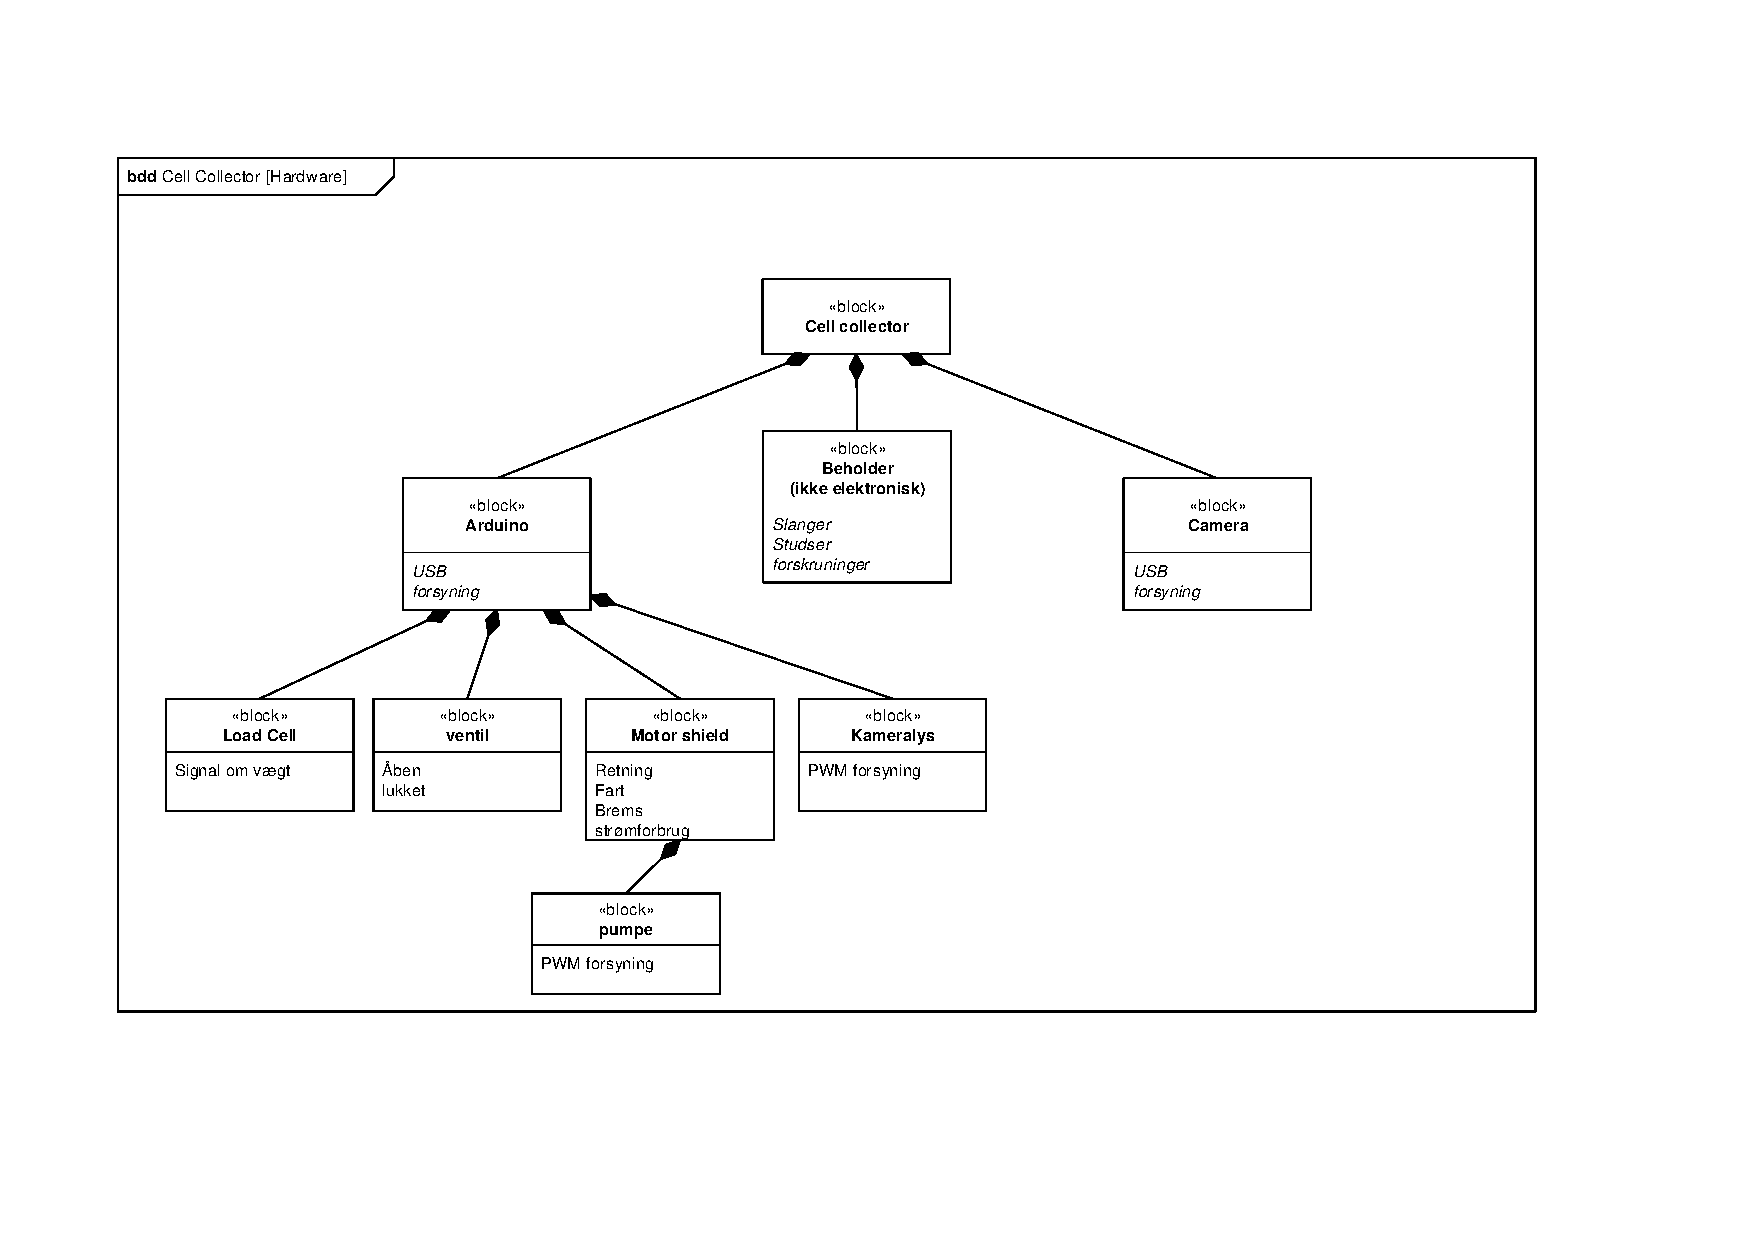
\includegraphics[width=1\textwidth]{pdf/BDD_Hardware.pdf}
	\caption{BDD - Cell Collector [Hardware]}
	\label{fig:bdd_Hardware}
\end{figure}

Nedenstående IBD figur \ref{fig:ibd_Hardware} beskriver mere præcist, hvordan de forskellige komponenter interagerer med hinanden på. Diagrammet er brugt til, at der tidligt i udviklingsforløbet bliver defineret hvilke spændinger og signaltyper systemet skal indeholde. Systemet skal indeholde bestemte typer for, at kunne kommunikere med de interne dele.


\begin{figure}[H]
	\centering
	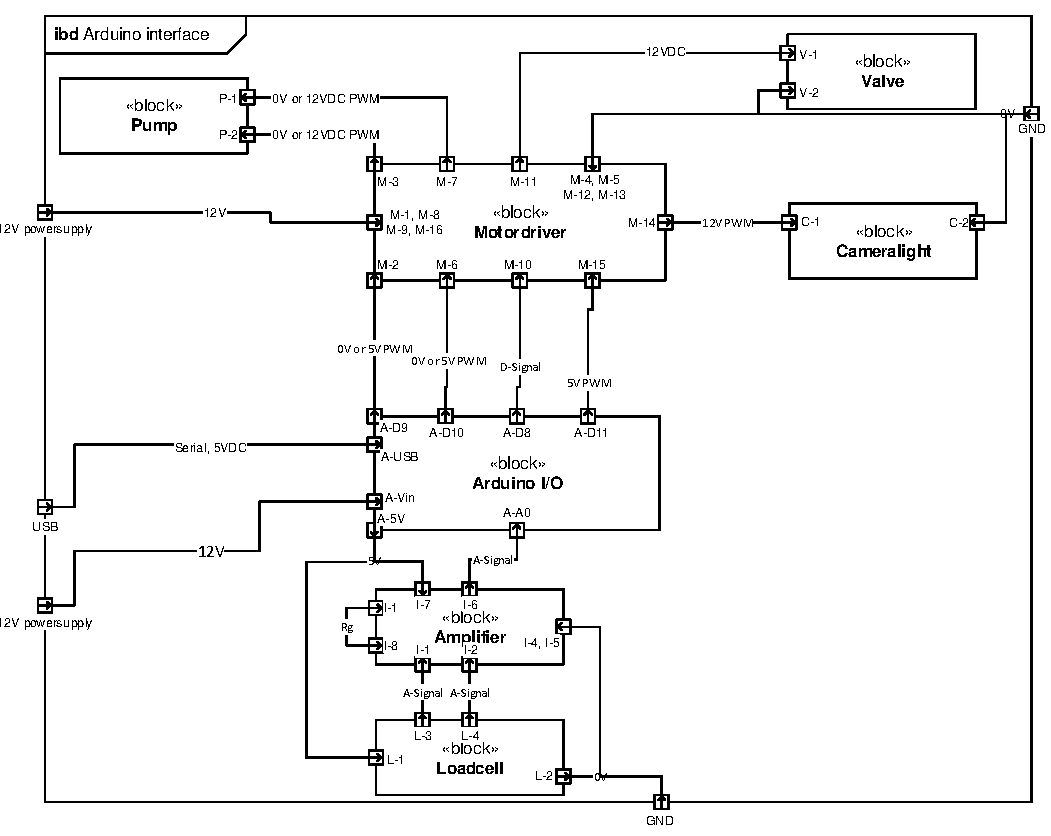
\includegraphics[width=1\textwidth]{pdf/IBD_Hardware(Arduino).pdf}
	\caption{IBD - Cell Collector [Hardware]}
	\label{fig:ibd_Hardware}
\end{figure}

Til ovenstående diagrammer er der udarbejdet tabeller som beskriver signalerne og de enkelte blokke. \fxnote{reference til projektdokumentation}

Derudover kan der ses specifikationerne for vægtcellen, og hvilke overvejelser der er gjort ved dette komponent.
\subsection{Vægtcelle}
\label{subsec:loadcell}
Vægtcellen skal bruges til at kontrollere om, der er væske i celleopløsningsbeholderen. Derfor når der ikke er mere væske i celleopløsningsbeholderen, stopper systemet sin sorteringscyklus.

\textbf{Specifikationer for Vægtcelle[\citet{DH7}]:} 
\begin{center}
		\begin{longtable}{ | m{6.5cm} | m{6.5cm}| } 
			\hline
			\textbf{Specifikation} &\textbf{Værdi} \\ 
			\hline
			\textbf{Max belastning:} & 1 kg \\ 
			\hline
			\textbf{Anbefalet arbejdsspænding} & 3-12V \\ 
			\hline
			\textbf{Output} & 1.0mV/V$\pm$0.15mV/V \\ 
			\hline
		\end{longtable}
\end{center}
---------------------------------------
Den indkøbte vægtcelle kan veje op til 1 kg, hvilket dækker vægten for celleopløsningsbeholderen på 250ml + beholderens vægt. I design fasen er der også beskrevet et teori afsnit for at dokumenter den opnået viden gruppe har fået, design afsnittet indeholder desuden også beregninger og kredsløbsdiagrammer. Det kan ses i den overstående tabel, at vægtcellens output er i millivolt hvilket har medført til at signalet skulle forstærkes. Dette er gjort vha. en operationsforstærker, for at vise et eksempel, er der trukket nedenstående ud fra design afsnittet se projektdokumentation afsnit XX \fxnote{reference} for hele afsnittet. 

I databladet \ref{bilag:INA114} til INA114 ses det at den har en CMRR på 115dB, ved et gain på 1000 og en indgangsmodstand på 10G$\Omega$. Forstærkningen kan regnes ud fra formlen i databladet \ref{eq:gainina1}
\begin{align}
 G=(1+\frac{50K\Omega}{R_{G}})
 \label{eq:gainina1}
 \end{align} 
 I dette projekt skal der bruges et gain på $\frac{4,9V}{5mV}=980$, 4,9V for ikke at komme i mætning på arduinoens ADC og 5mV da det er den maksimale spænding vægtcellen kan give, ved 5V forsyning.
 \begin{align}
 R_{G}=\frac{50k\Omega}{980-1}=51\Omega
 \label{eq:gainina2}
 \end{align}
Et gain på 980 giver en $NY_{Maksimalespænding}=980*5mV=4,9V \pm0,147V$, dvs at der nu er en opløsning på
\begin{align}
 \frac{1000g}{trin}=\frac{1000g}{1024}=0,977g/trin=>0,977*\frac{1024}{5V}=200g/V \pm30g
 \label{eq:gainina3}
 \end{align}
 
 Kredsløbet for INA114 og vægtcellen til arduinoen kan ses på figur \ref{fig:loadcelldiagram}
 
  \begin{figure}[H]
	\centering
	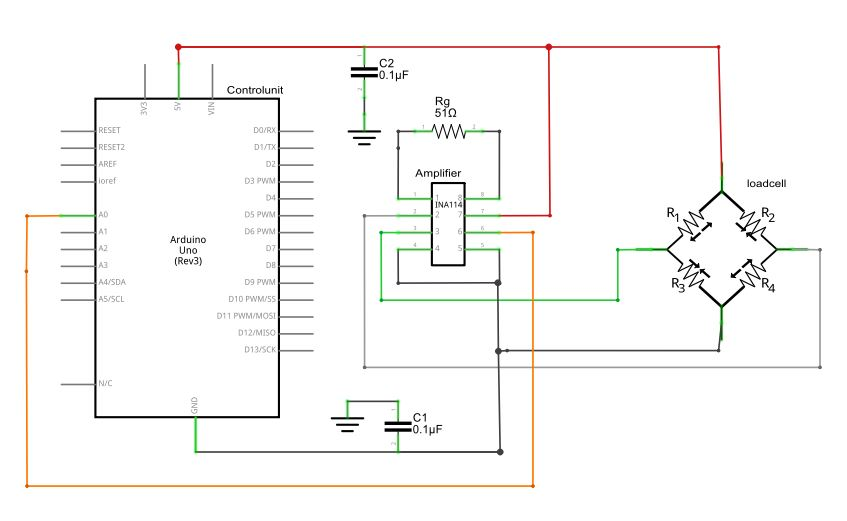
\includegraphics[width=0.9\textwidth]{billeder/Hardware/diagrammer/loadcelldiagram.JPG}
	\caption{Diagram for arduino, INA114 og vægtcelle}
	\label{fig:loadcelldiagram}
\end{figure}

\subsection{Sekvensdiagrammer}
Til sidst i design dokumentet er der lavet sekvensdiagrammer for, at få overblik over de sekventielle dele af systemet til hver use case se figur \ref{fig:sekvendisgr} for et eksempel. Sekvensdiagrammet har været en god måde for gruppen, at klargøre hvordan softwaren skal implementeres og i hvilken rækkefølge funktionerne her i skal eksekveres. Derudover har det været med til at danne et overblik over delene der skal implementeres i projektet, samt    dele opgaverne op i mindre opgaver.
\begin{figure}[H]
	\centering
	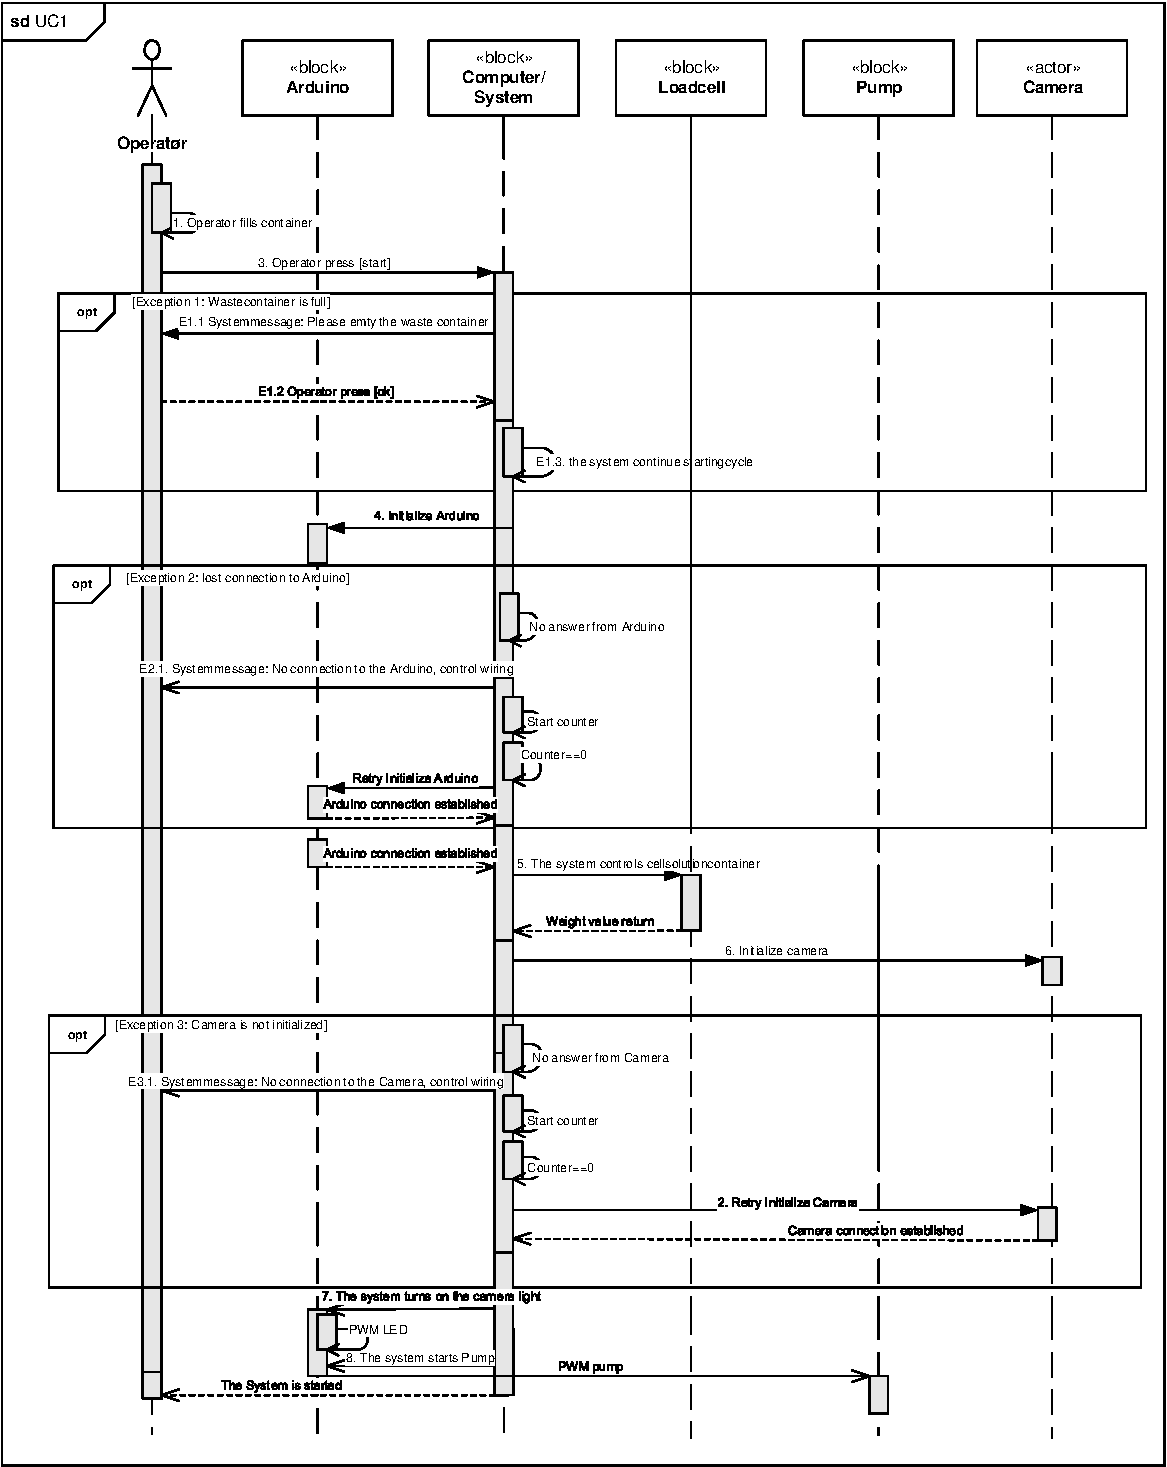
\includegraphics[width=1\textwidth]{pdf/UC1_cropped.pdf}
	\caption{Sekvensdiagram for usecase 1}
	\label{fig:sekvendisgr}
\end{figure}


\section{Implementering og enhedstest}
\label{subsec:Implement}
I dette afsnit er der vist et eksempel på hvordan delene er implementeret ved at vise vægtcellen for både hardware og software. Til sidst i denne fase er der lavet en integrationstest. Integrationstesten for hardwaren er bestået ved at lave et shield til arduinoen, \fxnote{skriv kameraet failede, men da det er en iterativ process har andre dele i projekt forsættes}

\subsection{Hardware}
Efter at diagrammet og kredsløbet blev udført i design dokumentet kunne vægtcellens kredsløb nu testes på et \textit{fumlebræt} 

Efter at diagrammet er fastlagt, testes forbindelserne nu på et \textit{fumlebræt} se figur \ref{fig:loadcelltest} for test opstilling

  \begin{figure}[H]
	\centering
	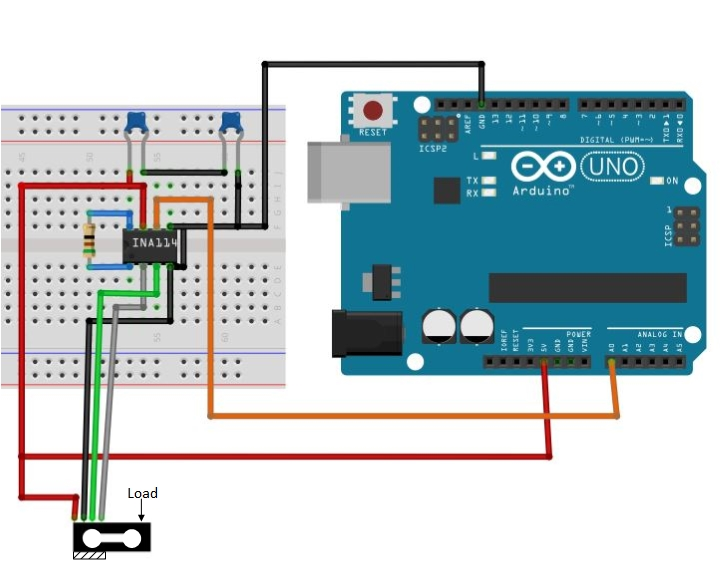
\includegraphics[width=0.9\textwidth]{billeder/Hardware/diagrammer/Drawing1.jpg}
	\caption{Test opstilling for vægtcelle}
	\label{fig:loadcelltest}
\end{figure}
De primære dele af test koden har været  \textit{sensorValue = analogRead(A0);} og \textit{Serial.println(sensorValue);}, hvor ved at inputtet på \textit{A0} er læst i \textit{serial monitor} som vist på figur \ref{fig:loadcell_test} ved langsom tømning af beholderen.

\begin{figure}[H]
	\centering
	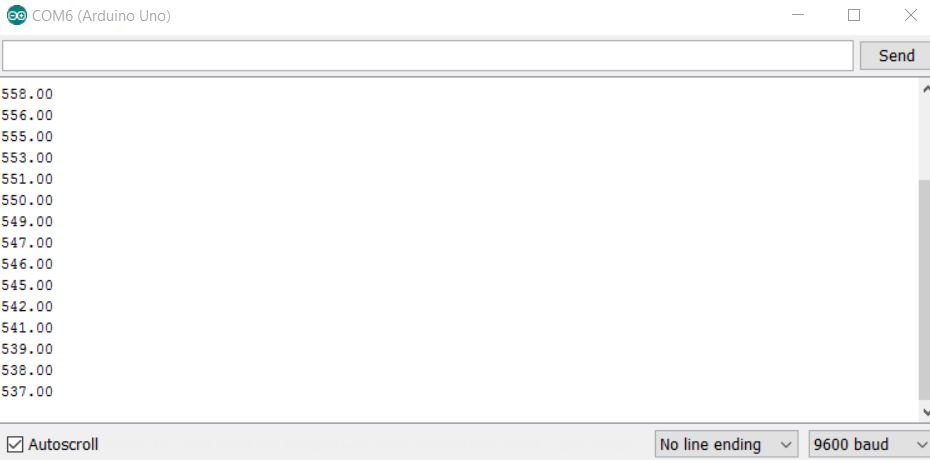
\includegraphics[width=0.9\textwidth]{billeder/Hardware/diagrammer/loadcellunittestbits.JPG}
	\caption{Værdier fra A0 i \textit{serial monitor}}
	\label{fig:loadcell_test}
\end{figure}

 Se bilag \ref{bilag:TKloadcell} for at se hele koden til testen. Til enhedstesten er der brugt et voltmeter til, at måle udgangsspændingen på INA114 for, at se om arduinoens ADC læste rigtigt. Til at sammenligne med voltmeteret, blev formlen \ref{eq:trintilvolt} brugt til at konvertere ADC'ens bits værdi om til spænding.
 
 \begin{align}
 analogRead(A_0)*\frac{5}{1024}=\text{spænding i volt}
 \label{eq:trintilvolt}
 \end{align}
Testopstilling af vægtcellen ser ud som på figur \ref{fig:loadcell_mont} med celleopløsningsbeholderen. I softwaren kræves det en kalibrering for at vægtcellen er præcis, dette er implementeret i projektdokumentation afsnit XX \fxnote{reference}.
 
 \begin{figure}[H]
	\centering
	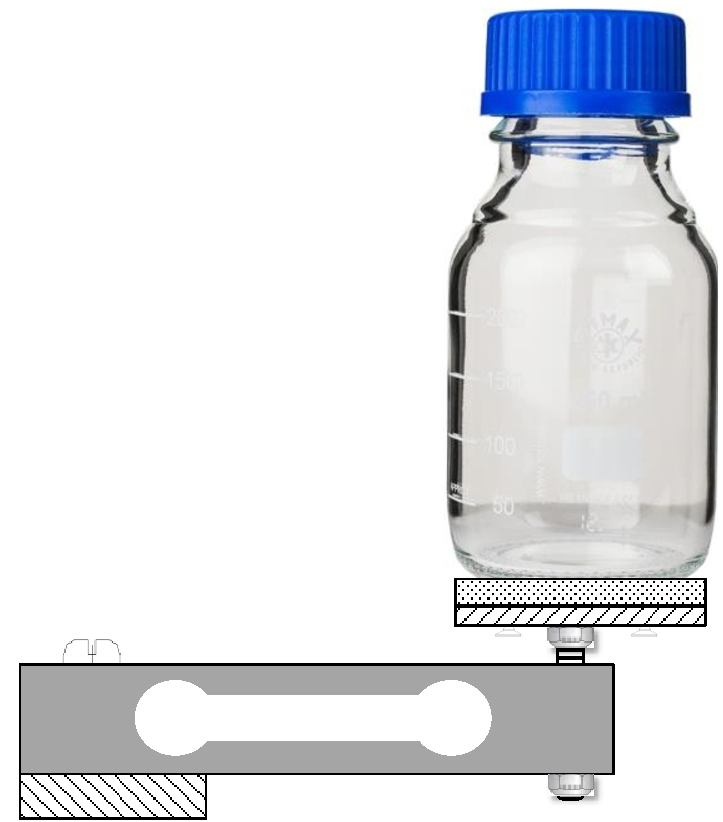
\includegraphics[width=0.5\textwidth]{billeder/Hardware/diagrammer/loadcell_montering.pdf}
	\caption{Illustration af opstilling med vægtcelle og celleopløsningsbeholder}
	\label{fig:loadcell_mont}
\end{figure}

\subsection{Kalibrering af vægtcellen}
Funktionen til vægt cellen er implementeret efter beskrivelsen i design dokumentet i projektdokumentation afsnit XX. Dens funktion er, at konvertere det analoge input (V) til indholdet (ml) i celleopløsningsbeholderen. Dette er implementeres ved en lineær model:
\begin{align}
mL = a*input+b \text{, hvor a er hældningen og b er skæringen med y aksen}
\end{align}
Det analoge input ganges altså med en faktor \textit{a} plus et offset \textit{b} for at konvertere spænding til antal ml. Nedenstående tabel viser indgangsspændingen for forskellige mængder i beholderen. Udfra disse data er der lavet en lineær regression for at finde hældningen \textit{a} og skæringen \textit{b}.
\begin{center}
		\begin{longtable}{ | m{3cm} | m{3cm}| } 
			\hline
			\textbf{ml i beholder} &\textbf{Analog input} \\ 
			\hline
			 \SI{0}{\milli\litre} & \SI{1.9487}{\volt} \\ 
			\hline
			 \SI{25}{\milli\litre} & \SI{2.0440}{\volt} \\ 
			\hline
			\SI{50}{\milli\litre} & \SI{2.1320}{\volt} \\ 
			\hline
			\SI{75}{\milli\litre} & \SI{2.2297}{\volt} \\ 
			\hline
			\SI{100}{\milli\litre} & \SI{2.3109}{\volt} \\ 
			\hline
			\SI{125}{\milli\litre} & \SI{2.4071}{\volt} \\ 
			\hline
			\SI{150}{\milli\litre} & \SI{2.4961}{\volt} \\ 
			\hline
			\SI{175}{\milli\litre} & \SI{2.5821}{\volt} \\ 
			\hline
			\SI{200}{\milli\litre} & \SI{2.6760}{\volt} \\ 
			\hline
			\SI{225}{\milli\litre} & \SI{2.7654}{\volt} \\ 
			\hline
			\SI{250}{\milli\litre} & \SI{2.8587}{\volt} \\ 
			\hline
			\caption{Kalibreringsdata for vægtcellen}
			 		\end{longtable}
\end{center}

I Matlab er funktionen \textit{fitlm} anvendt til at finde det bedste lineære fit. Regressionen er baseret på Least Square metoden. \fxnote{Henvisning}
Udfra beregningerne i Matlab er hældningen a og skæringen b fundet til hhv:
\begin{align}
a = 276.14
\end{align}
\begin{align}
b = -539.02
\end{align}
Den endelige funktion er dermed givet ved:
\begin{align}
ml = 276.140*input-539.02
\end{align}

Figur \ref{fig:loadcellcalib} viser den lineære funktion, samt de enkelte data punkter fra tabellen. 
\begin{figure}[H]
	\centering
	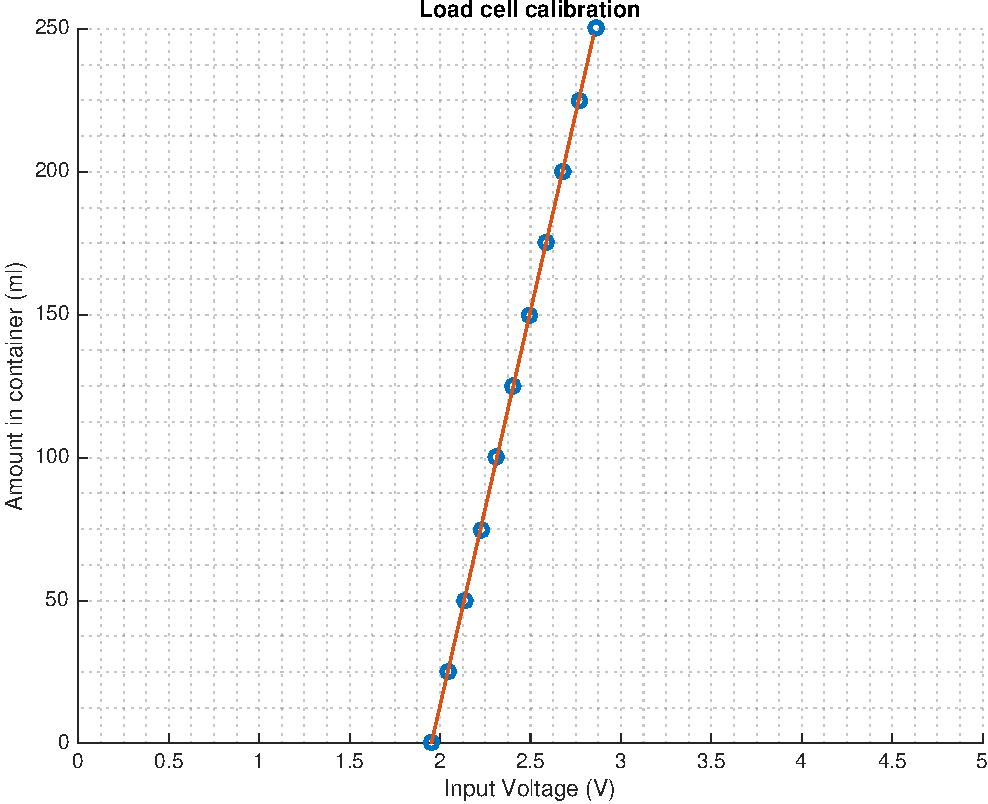
\includegraphics[width=0.6\textwidth]{billeder/software/calibration-crop.pdf}
	\caption{Kalibrering af load cell}
	\label{fig:loadcellcalib}
\end{figure}

For at reducere støj og mindske følsomheden overfor hurtigere ændringer i indgangsspændingen er der implementeret en midling af de seneste 10 målinger. Dette er med til, at gøre konverteringen mere robust overfor støj. 

\subsection{Integrationstest}
Til sidst i denne fase er der udført en integrationstest, hvor hardwaren er samlet, efter alle enkle enhedstest er udførte. Efter samlingen af hardwaren og verificeret at kredsløbet virker, er der designet et PCB til samlingen af hardwaren. Derefter er integrationen med softwaren sket og igen er det verificeret, at det fungerer til en færdig prototype. 

